\section{Existing Systems}

Several freelance platforms currently dominate the digital labour market. This section reviews the four platforms that are closest to FREVIA---Upwork, Fiverr, Freelancer, and Toptal---and then positions the proposed system against them. For each platform, the review examines its operational scope, its main features, its core strengths, and its concrete limitations. Crucially, each limitation is analysed with respect to the specific problems it creates for users and the exact technical mechanisms through which FREVIA addresses or resolves those problems.

\subsection{Upwork}

\begin{figure}[H]
\centering

\includegraphics[width=0.85\textwidth]{image/existing/upwork.png}
\caption{Upwork -- illustrative screenshot of the existing platform}
\label{fig:existing-upwork}
\end{figure}

\begin{itemize}[leftmargin=*]
\item \textbf{Overview:} Upwork is a global freelance marketplace where clients publish jobs and freelancers submit proposals for hourly or fixed-price contracts.
\item \textbf{Link:} \url{https://www.upwork.com}
\item \textbf{Main features:} Job posting, proposal submission, hourly and fixed-price contracts, milestone escrow, work diaries, direct messaging, client reviews, and payment protection.
\item \textbf{Strengths:} A massive global user base, an established enterprise reputation system, verified payment methods, and an end-to-end contract-to-payment workflow.
\item \textbf{Limitations and Concrete Problem Analysis:}
    \begin{itemize}[leftmargin=*]
        \item \textbf{Specific Problem 1 (High Double-Sided Commission Fees):} Upwork charges a 10\% service fee on freelancer earnings alongside an additional 5\% client marketplace fee on every transaction. For long-term or high-value contracts, this substantial percentage take-rate significantly diminishes freelancer income and inflates project costs for clients.\\
        $\rightarrow$ \textbf{FREVIA Resolution:} FREVIA replaces percentage-based revenue cuts with a transparent, flat platform fee per contract (\$5 fixed fee charged to the client upon contract creation). Freelancers receive 100\% of their milestone earnings without ongoing commission deductions.
        \item \textbf{Specific Problem 2 (Overwhelming Manual Proposal Screening):} High-demand postings routinely receive dozens or hundreds of bids, forcing clients to manually read through unstandardised cover letters and unformatted attachments, leading to hiring fatigue and slow turnaround times.\\
        $\rightarrow$ \textbf{FREVIA Resolution:} FREVIA integrates an automated AI CV Analysis pipeline. When freelancers apply, the AI parses candidate resumes, extracts structured technical skills and experience levels, and calculates a semantic match score against the job requirements, allowing clients to shortlist top talent immediately.
        \item \textbf{Specific Problem 3 (Account Impersonation and Fraudulent Identities):} Despite automated checks, account renting, credential sharing, and fabricated identities remain prevalent on open bidding platforms.\\
        $\rightarrow$ \textbf{FREVIA Resolution:} FREVIA enforces a rigorous multi-step identity verification module combining national ID (CCCD/Passport) OCR document extraction with automated facial liveness verification, subject to mandatory platform administrator audit before issuing verified freelancer badges.
    \end{itemize}
\end{itemize}

\subsection{Fiverr}

\begin{figure}[H]
\centering

\includegraphics[width=0.85\textwidth]{image/existing/fiverr.png}
\caption{Fiverr -- illustrative screenshot of the existing platform}
\label{fig:existing-fiverr}
\end{figure}

\begin{itemize}[leftmargin=*]
\item \textbf{Overview:} Fiverr is a service catalogue built from predefined packages, called gigs, in which freelancers publish a fixed scope and buyers purchase directly without prior bidding.
\item \textbf{Link:} \url{https://www.fiverr.com}
\item \textbf{Main features:} Gig packages with tiered pricing (Basic, Standard, Premium), direct checkout, order requirements, in-order messaging, delivery and revision cycles, and public review ratings.
\item \textbf{Strengths:} Extremely low friction for buyers seeking standard tasks, transparent pricing, fast ordering, and a catalogue model that eliminates protracted proposal review.
\item \textbf{Limitations and Concrete Problem Analysis:}
    \begin{itemize}[leftmargin=*]
        \item \textbf{Specific Problem 1 (Rigid Pre-Packaged Scope Unfit for Complex Projects):} Static gig packages cannot accommodate evolving software architectures, multi-phase technical specifications, or projects requiring customized requirements negotiation.\\
        $\rightarrow$ \textbf{FREVIA Resolution:} FREVIA abandons rigid gig packages in favour of custom job postings and proposal submissions. Clients define precise project specifications, and freelancers negotiate tailored scopes, deliverable schedules, and custom contract term templates.
        \item \textbf{Specific Problem 2 (Absence of Milestone-Based Staged Escrow):} Fiverr treats orders as single lump-sum transactions. Large projects cannot be segmented into sequential funded milestones, creating substantial financial risk for buyers and preventing progressive deliverable approvals.\\
        $\rightarrow$ \textbf{FREVIA Resolution:} FREVIA implements Milestone-based Escrow funding via Stripe. Contracts are divided into distinct milestones, each backed by dedicated escrow funding that is released only after client review and formal acceptance of each milestone deliverable.
        \item \textbf{Specific Problem 3 (Restricted Contract Term Negotiation and Legal Protection):} Standard Fiverr transactions lack mutual legal agreements, custom intellectual property (IP) transfer terms, or non-disclosure agreements (NDAs).\\
        $\rightarrow$ \textbf{FREVIA Resolution:} FREVIA provides customizable contract term templates with formal dual-signature acceptance, establishing enforceable IP transfer, confidentiality commitments, and explicit milestone deadlines prior to fund deposit.
    \end{itemize}
\end{itemize}

\subsection{Freelancer}

\begin{figure}[H]
\centering
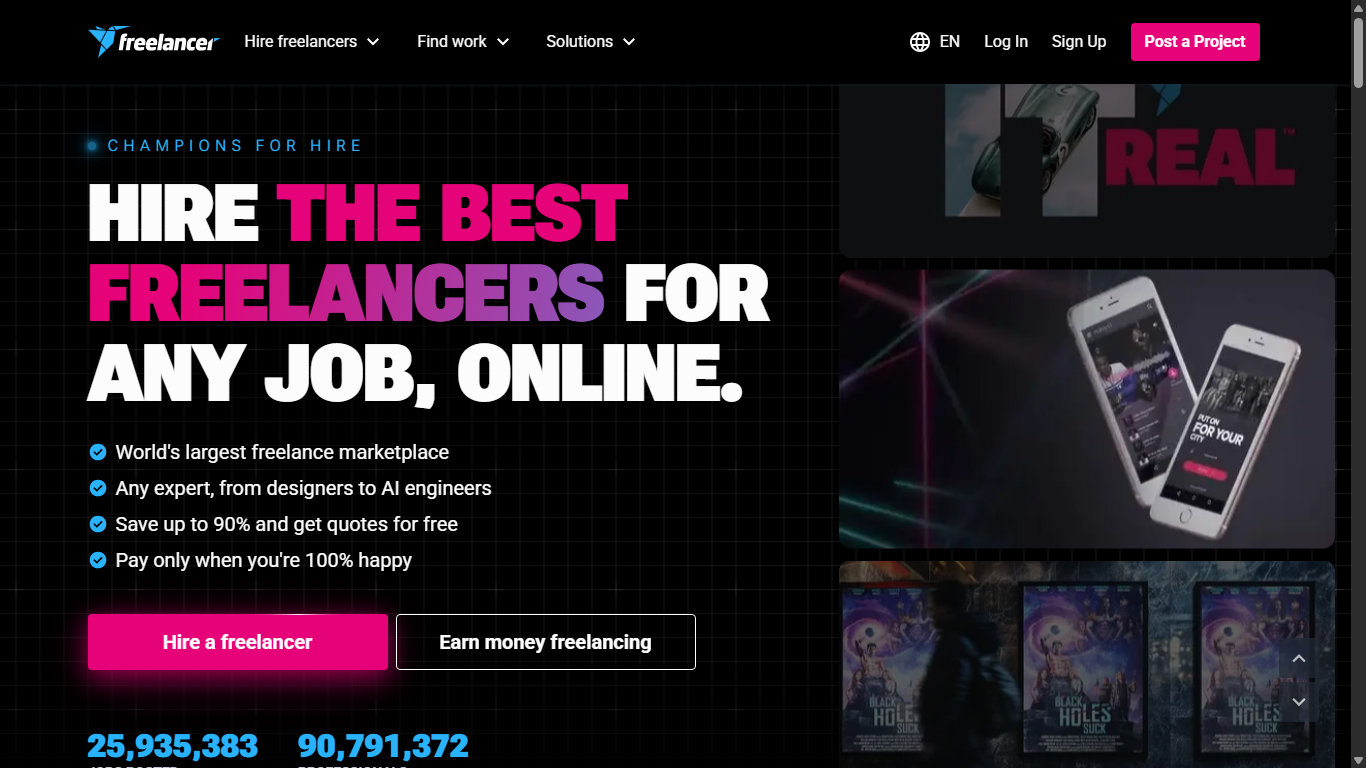
\includegraphics[width=0.85\textwidth]{image/existing/freelancer.png}
\caption{Freelancer -- illustrative screenshot of the existing platform}
\label{fig:existing-freelancer}
\end{figure}

\begin{itemize}[leftmargin=*]
\item \textbf{Overview:} Freelancer is a large-scale project marketplace supporting competitive bidding, crowdsourced design contests, and milestone-based payments across global categories.
\item \textbf{Link:} \url{https://www.freelancer.com}
\item \textbf{Main features:} Project bidding, design contests, milestone escrow payments, internal messaging, preferred freelancer programs, and dispute resolution.
\item \textbf{Strengths:} Broad category coverage, high bid volume providing diverse price points, and globally accessible milestone escrow capabilities.
\item \textbf{Limitations and Concrete Problem Analysis:}
    \begin{itemize}[leftmargin=*]
        \item \textbf{Specific Problem 1 (High Volume of Low-Quality and Automated Bot Bids):} Job postings are instantly inundated with copy-paste proposals from automated bots, drowning out genuine subject-matter experts and forcing clients to sift through spam.\\
        $\rightarrow$ \textbf{FREVIA Resolution:} FREVIA combats bid spam by requiring verified identity credentials before proposal submission, enforcing proposal drafting limits, and applying AI proposal relevance scoring to highlight genuine, customized responses.
        \item \textbf{Specific Problem 2 (Opaque, Costly, and Rigid Dispute Arbitration):} Freelancer charges heavy dispute fees (\$25 or 5\%) and adjudicates conflicts behind closed doors through internal support staff without structured evidence sharing or transparent appeals.\\
        $\rightarrow$ \textbf{FREVIA Resolution:} FREVIA provides a transparent 5-stage Dispute Arbitration workflow: (1) Dispute Filing with milestone lock, (2) Structured evidence and attachment submission, (3) Formal platform administrator evaluation, (4) Proportionate escrow allocation (full release, full refund, or split decision), and (5) Dispute Decision Review (formal appeal stage) with a complete audit trail.
    \end{itemize}
\end{itemize}

\subsection{Toptal}

\begin{figure}[H]
\centering
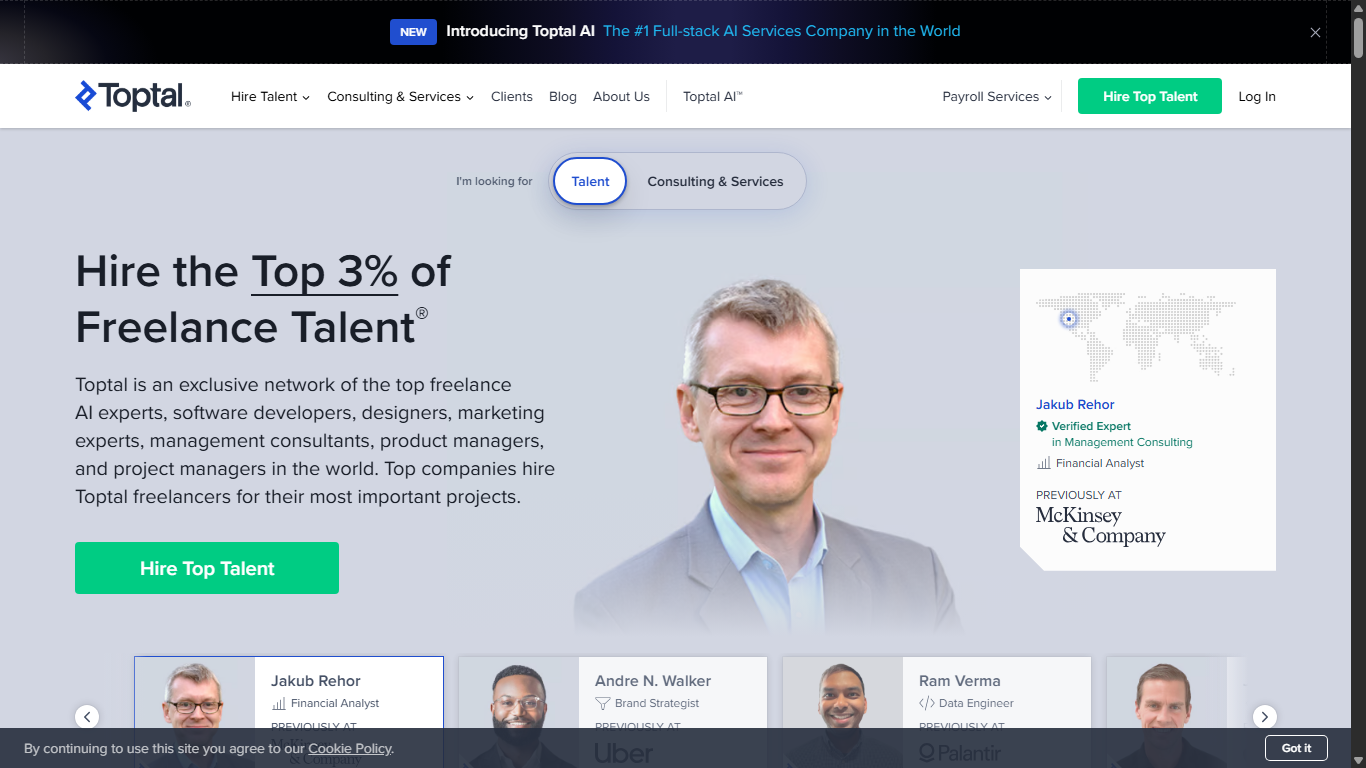
\includegraphics[width=0.85\textwidth]{image/existing/toptal.png}
\caption{Toptal -- illustrative screenshot of the existing platform}
\label{fig:existing-toptal}
\end{figure}

\begin{itemize}[leftmargin=*]
\item \textbf{Overview:} Toptal is an exclusive talent network that screens applicants rigorously (accepting only the ``top 3\%'') and matches clients with pre-vetted specialists via dedicated platform account managers.
\item \textbf{Link:} \url{https://www.toptal.com}
\item \textbf{Main features:} Multi-tier applicant vetting (language proficiency, technical problem solving, live coding, trial projects), account-manager matching, and enterprise invoicing.
\item \textbf{Strengths:} Exceptionally high talent quality, near-zero hiring risk for enterprise clients, and curated matches that save client screening time.
\item \textbf{Limitations and Concrete Problem Analysis:}
    \begin{itemize}[leftmargin=*]
        \item \textbf{Specific Problem 1 (Extreme Barrier to Entry Excluding Qualified Professionals):} The rigid 3\% acceptance quota excludes the vast majority of skilled, capable freelancers who do not pass specialized automated algorithms or multi-month screening funnels.\\
        $\rightarrow$ \textbf{FREVIA Resolution:} FREVIA operates an open, merit-based marketplace accessible to all legitimate professionals, while introducing a distinct ``Verified Expert'' tier and public directory to spotlight elite vetted talent without barring emerging freelancers.
        \item \textbf{Specific Problem 2 (Prohibitive Pricing and Enterprise Bias):} High hourly billing rates (\$60--\$200+/hour) and substantial initial deposits make Toptal inaccessible to startups, small businesses, and budget-constrained project owners.\\
        $\rightarrow$ \textbf{FREVIA Resolution:} FREVIA democratises professional contracting by supporting flexible fixed-price projects across all budget tiers, empowering clients to negotiate directly with talent based on project requirements.
        \item \textbf{Specific Problem 3 (Centralized Platform Matching Without Direct Client Autonomy):} Clients cannot independently search, compare, or select candidate proposals; all hiring decisions are mediated by Toptal account managers.\\
        $\rightarrow$ \textbf{FREVIA Resolution:} FREVIA restores full client autonomy: clients post jobs, review comprehensive proposals, inspect portfolios, interact directly via real-time messaging, and retain total control over hiring decisions.
    \end{itemize}
\end{itemize}

\subsection{FREVIA (Proposed System)}

\begin{itemize}[leftmargin=*]
\item \textbf{Overview:} FREVIA is a web-based freelance marketplace that places verification, escrow, and project governance at the centre of the transaction rather than treating them as optional add-ons.
\item \textbf{Main features:} Email and Google authentication with one-time-code verification; multi-role accounts with a dynamic, database-driven RBAC permission model; freelancer, client, and expert profiles with administrative revision approval; AI-assisted identity verification (national ID OCR and facial liveness check); job posting with fixed-price budgets and multiple hiring positions; proposals with drafts and expiry; dual-signed contracts with a fixed flat platform fee; milestone funding and release through Stripe Escrow; escrow-backed dispute arbitration with formal review; contract reviews with responses; one-to-one real-time messaging; in-app notifications; an AI-moderated community forum; and announcement/advertisement banners.
\item \textbf{Strengths:} 
    \begin{itemize}[leftmargin=*]
        \item \textbf{Governance and Escrow by Design:} Milestone escrow is integral to every contract; money is deposited before work starts and released only upon explicit deliverable sign-off.
        \item \textbf{AI-Assisted Efficiency:} Resume skill parsing, candidate match scoring, and identity document verification significantly accelerate hiring while maintaining safety.
        \item \textbf{Transparent Arbitration:} Disagreements follow a structured 5-stage legal workflow with evidence submission, escrow partitioning, and formal appeal capabilities.
        \item \textbf{Cost Fairness:} A single flat platform fee per contract eliminates high percentage commission deductions.
    \end{itemize}
\item \textbf{Limitations and Boundaries:}
    \begin{itemize}[leftmargin=*]
        \item \textbf{Cold-Start User Base:} As a new platform, FREVIA lacks the massive established liquidity and user network of Upwork or Fiverr; initial adoption requires strategic recruitment.
        \item \textbf{Payment Boundary:} Payouts and onboarding rely strictly on Stripe Connect supported countries; domestic e-wallets, direct local bank rails, and cryptocurrency settlements are outside the current scope.
        \item \textbf{Fixed-Price Contract Model:} Only fixed-price milestone contracts in USD are supported; hourly billing and automated background screen-recording surveillance are intentionally excluded.
    \end{itemize}
\end{itemize}

\subsection{Comparative Analysis Matrix}

Table~\ref{tab:existing-comparison} synthesises the operational differences between the four established platforms and FREVIA, illustrating the strategic gap that the proposed system addresses.

\begin{table}[H]
\centering
\footnotesize
\setlength{\tabcolsep}{4pt}
\begin{tabularx}{\textwidth}{|>{\bfseries}p{2.8cm}|X|X|X|X|p{2.8cm}|}
\hline
\rowcolor{fptHeader}\textcolor{fptHeaderText}{\textbf{Dimension}} & \textcolor{fptHeaderText}{\textbf{Upwork}} & \textcolor{fptHeaderText}{\textbf{Fiverr}} & \textcolor{fptHeaderText}{\textbf{Freelancer}} & \textcolor{fptHeaderText}{\textbf{Toptal}} & \textcolor{fptHeaderText}{\textbf{FREVIA}} \\ \hline
Marketplace Model & Open bidding & Predefined gigs & Bidding \& contests & Curated network & Open bidding + Expert directory \\ \hline
Fee Structure & 10\% + 5\% & 20\% + 5.5\% & 10\% + 3\% & High enterprise markup & Flat \$5 / contract \\ \hline
Milestone Escrow & Supported & Not supported (Lump-sum) & Supported & Hourly / Weekly billing & Full Stripe Milestone Escrow \\ \hline
Scope Negotiation & High & Very limited & High & High & Full with Contract Term Templates \\ \hline
Dispute Process & Internal mediation & Support ticket & Paid opaque arbitration & Account manager & 5-Stage evidence arbitration + appeals \\ \hline
Identity Vetting & ID check & Minimal & Optional KYC & Multi-month top 3\% testing & AI OCR + Facial liveness + Admin audit \\ \hline
Candidate Screening & Manual cover letters & Catalogue ratings & Manual bid filtering & Platform recruiter & AI CV extraction \& match score \\ \hline
Client Autonomy & Direct hiring & Direct purchase & Direct hiring & Delegated matching & Direct hiring with AI assistance \\ \hline
\end{tabularx}
\caption{Comparative feature matrix between existing platforms and FREVIA}
\label{tab:existing-comparison}
\end{table}

\noindent\textbf{Summary of Differentiators:} The analysis shows that FREVIA does not attempt to reinvent milestone escrow or basic bidding, which are already present on Upwork and Freelancer. Instead, FREVIA addresses the concrete limitations of existing systems by delivering: (1) a transparent arbitration procedure with formal appeals and evidence disclosure, (2) an accessible flat-fee economic model that does not penalise freelancer earnings, (3) automated AI CV analysis to eliminate manual screening fatigue, and (4) an open marketplace that combines verified identity integrity with full client hiring autonomy.
